\documentclass[letter]{bioinfo}
\copyrightyear{2018} \pubyear{2018}
\usepackage{soul} %highlight stuff

%bibliography magic
\usepackage{natbib}
\setlength{\bibsep}{\baselineskip} %dbl space between citations

\usepackage{hyperref}
\access{Advance Access Publication Date: (under review)}
\appnotes{Review article}
\graphicspath{{../figures/}}

\newcommand{\comment}[1]{\textcolor{red}{[#1]}}
\newcommand{\todo}[1]{\colorbox{yellow}{\parbox{1\linewidth}{#1}}}


\begin{document}
	\firstpage{1}
	
	\subtitle{Review}
	
	\title[Cardioinformatics]{Cardioinformatics: the nexus of bioinformatics and cardiology}
	\author[Khomtchouk \textit{et~al}.]{Bohdan B. Khomtchouk\,$^{\text{\sfb 1,2,3,}*,$\dag$}$,\, Diem-Trang Tran\,$^{\text{\sfb 4},$\dag$}$, Kasra A. Vand\,$^{\text{\sfb 5}}$, Or Gozani\,$^{\text{\sfb 1}}$, Matthew Might\,$^{\text{\sfb 6}}$, Themistocles L. Assimes\,$^{\text{\sfb 2, 3}}$}
	\address{$^{\text{\sf 1}}$Department of Biology, Stanford University, Stanford, CA, USA \\
		$^{\text{\sf 2}}$Department of Medicine, Division of Cardiovascular Medicine, Stanford University, Stanford, CA, USA \\
		$^{\text{\sf 3}}$VA Palo Alto Health Care System, Palo Alto, CA, USA \\
		$^{\text{\sf 4}}$School of Computing, University of Utah, Salt Lake City, UT, USA \\
		$^{\text{\sf 5}}$Quiltomics, Palo Alto, CA, USA \\
		$^{\text{\sf 6}}$Hugh Kaul Personalized Medicine Institute, University of Alabama at Birmingham, Birmingham, AL, USA \\
	}
	
	\corresp{$^\ast$To whom correspondence should be addressed: \href{bohdan@stanford.edu}{bohdan@stanford.edu}\\
	$^\dagger$These authors contributed equally to this work.
	}

	
	\history{Received on XXXXX; revised on XXXXX; accepted on XXXXX}
	
	\editor{Associate Editor: XXXXXXX}
	
	\abstract{Cardiovascular disease (CVD) is the leading cause of death worldwide, causing over 17M deaths per year, which outpaces global cancer mortality rates.  Despite these sobering statistics, most bioinformatics and computational biology work to-date has been concentrated predominantly on cancer research, with a relatively modest footprint in CVD.  In this paper, we review the existing literary landscape and critically assess the unmet need to further develop an emerging field at the multidisciplinary interface of bioinformatics and cardiovascular medicine, which we refer to as "cardioinformatics".  To promote reproducibility, all data and source code powering the data-driven visualizations and quantitative analyses presented in this review are provided at: https://github.com/Bohdan-Khomtchouk/cardioinformatics. \\
		\textbf{Keywords:} cardiovascular disease; bioinformatics; cardiology; computational biology}
	
\maketitle
	
\section*{Introduction}
	%\section*{The current status of bioinformatics in cardiovascular disease research}
	
Cardiovascular diseases have persistently been the leading cause of death by communicable and non-communicable diseases in the US for the last many decades (Figure \ref{fig:figure1}A).  According to the World Health Organization, ischemic heart disease and stroke have remained the top two global killers in the last 15 years. The Global Burden of Diseases, Injuries, and Risk Factors Study shows that while heart disease and cancer have similar mortality rates in the US, heart disease is still the dominant cause of death globally for both genders \citep{Roth:2018:Global}.  Research in CVD has steadily increased since the year 2000, as measured by the body of publications indexed in PubMed over this time (Figure \ref{fig:figure1}B).  In 2017 alone, there were more than 40000 primary research (non-review) articles classified with the subject heading "cardiovascular disease", defined according to the Medical Subject Heading (MeSH) terms.  This MeSH Database entry (\textit{cardiovascular disease}) includes many types of cardiovascular abnormalities that may occur in organs outside the immediate circulatory system, highlighting the complex disease nature of CVD.


\begin{figure}[!tpb]
	\centering
	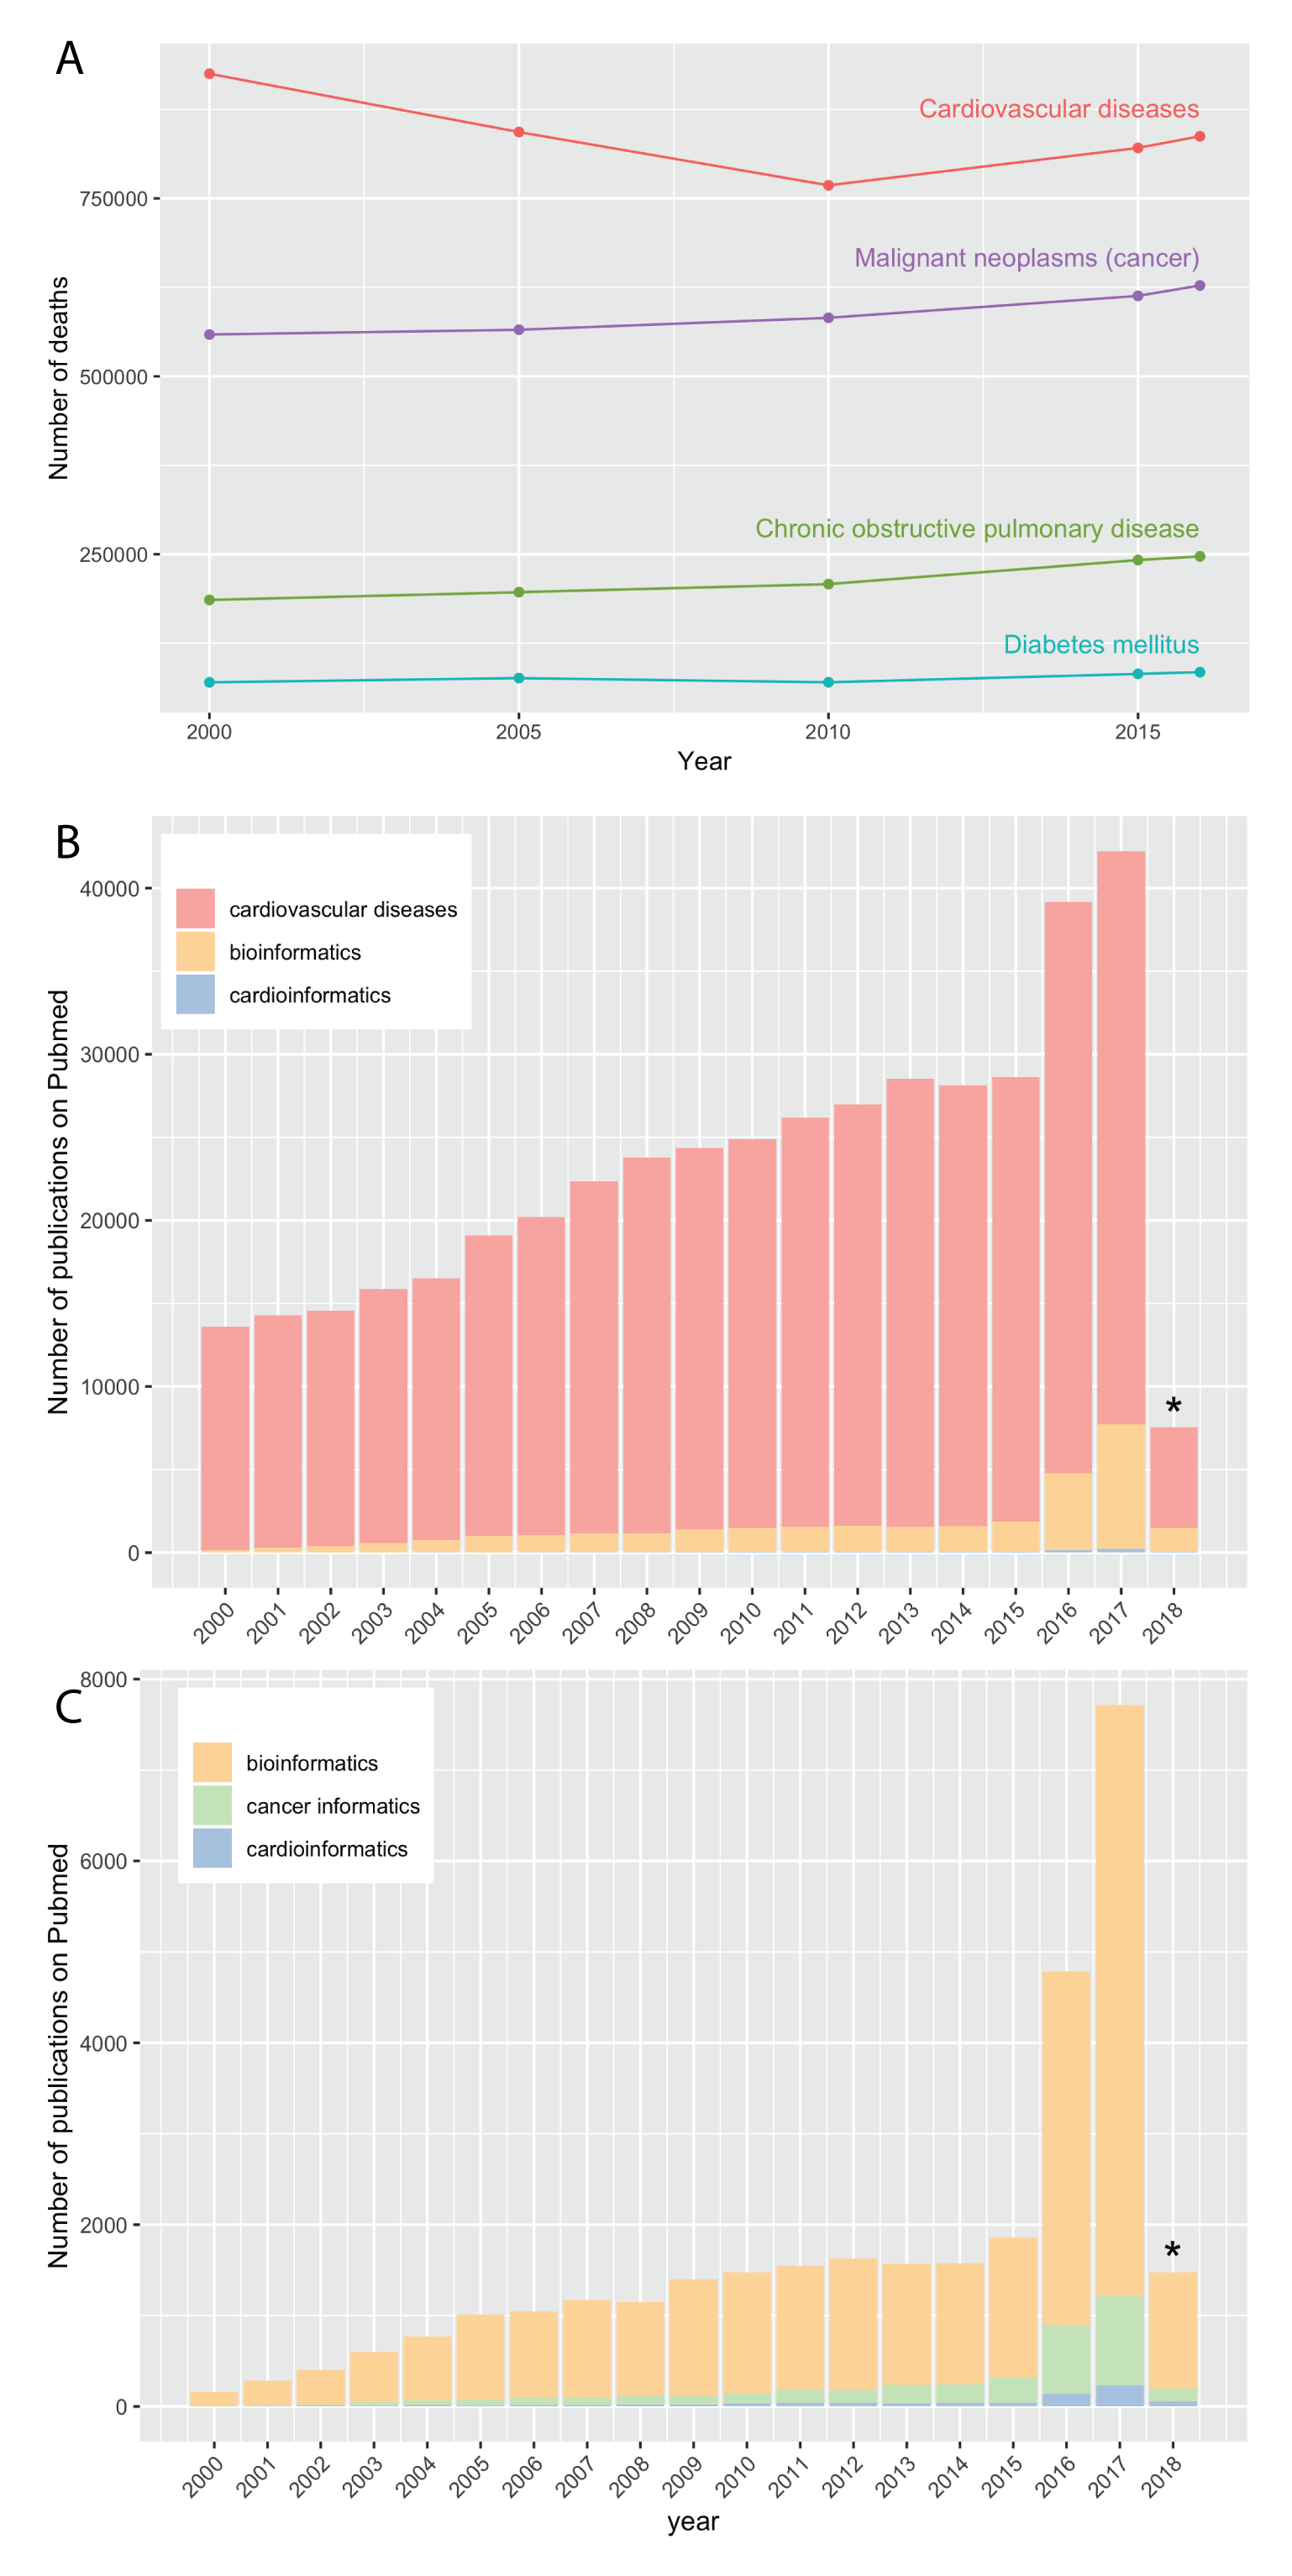
\includegraphics[width=1\linewidth]{figure1}
	\caption{\textbf{(A)} Number of deaths by Non-Communicable Diseases in the US.  Cardiovascular disease deaths have consistently surpassed cancer mortality rates since at least the year 2000.  \textbf{(B)} Text mining PubMed reveals that out of the total body of CVD research published in peer-reviewed journals, only a vanishingly small percentage include bioinformatics techniques or methodologies as part of the study design.  Likewise, there are far more CVD papers released annually than bioinformatics papers (in any domain area, not just CVD), highlighting the tremendous momentum and volume of new research results published in the CVD field.  Nevertheless, only a small percentage of that total CVD literature includes bioinformatics techniques.  \textbf{(C) Relative to the total pool of bioinformatics papers (in any field), there are far more cancer papers that utilize bioinformatics methods than CVD papers that utilize such methods.}\\
	* Since all the queries are based on manual MeSH catalog, 2018 tallies will lag behind the true volume of publication.}
	\label{fig:figure1}
\end{figure}


The share of bioinformatics research has remained modest among these CVD outputs at least relative to comparable work done in cancer biology (Figure \ref{fig:figure1}C). While bioinformatics is at the center of precision medicine \citep{Gomez-Lopez:2017:Precision} and cardiovascular research is at the forefront of existing precision medicine initiatives \citep{Houser:2016:American,czbiohub:2018:Chan}, the field of cardioinformatics is still in its early days with ample opportunities to benefit from cutting-edge data science techniques and machine learning (ML) methodologies, as has been the case in oncology.  Even now, the application of ML is already being recognized as an indispensable component of the practice of cardiology in the future \citep{Shameer:2017:Translational,Shameer:2018:Machine} and, therefore, given the availability of increasingly performant ML implementations \citep{MLPerf:2018:MLPerf}, cardioinformatics is better positioned to tackle domain-specific research questions by developing clinical applications to enhance compute-intensive tasks such as those found in medical imaging, CVD risk prediction modeling, among other active research areas. In general, efficient implementations of advanced computational algorithms that optimize for time, cost, and accuracy measures across broad domains of biological data science, such as single-cell sequencing \citep{Becht:2018:Evaluation} or long-read mapping \citep{Li:2018:Minimap2}, will find increasingly more adoption in CVD research throughout the next few years as journals begin gearing up for the release of special issues dedicated exclusively to performance benchmarking of new and existing software tools.  In addition, the availability of open-access benchmarking data and guidelines to evaluate ML methods across a broad range of application areas including biomedical studies, signal processing and image classification, will catalyze the precipitation of the best bioinformatics software tools to the top \citep{Olson:2017:PMLB,Weber:2018:Essential}.  Taken together, programmatic need for bioinformatics benchmarking and awareness of state-of-the-art tools for performing CVD research will bridge across multiple areas of expertise (e.g., single-cell sequencing technologies, long-read mapping, 3D genome visualization, etc.), making cardioinformatics research a truly multi-disciplinary initiative for dissecting the molecular mechanisms behind complex CVD traits.   


The American Heart Association (AHA) Institute for Precision Cardiovascular Medicine recently partnered with Amazon Web Services to provide a variety of grant funding opportunities for testing and refining artificial intelligence (AI) and ML algorithms using healthcare system data and multiple longitudinal data sources to fund research that improves our understanding of all CVD data related to precision medicine.  Therefore, we expect that grant funding initiatives such as these will gradually begin narrowing the gap between cardioinformatics and cancer research in terms of the availability of improved computational tools, infrastructure, and analysis resources.  Some recent positive trends in this direction include large-scale infrastructure and knowledge portal development \citep{Kass-Hout:2018:American, Khomtchouk:2018:HeartBioPortal, Broad:NA:Cardiovascular, Broad:NA:Cerebrovascular} for working with CVD data, as well as population-wide multi-omics initiatives such as the NHLBI Trans-Omics for Precision Medicine (TOPMed) Consortium \citep{NHLBI:2014:TransOmics} for integrating whole-genome sequencing (WGS) and other -omics data (e.g., metabolic profiles, protein and RNA expression patterns) with molecular, behavioral, imaging, environmental, and clinical data.  In this review, we highlight these contemporary opportunities and perspectives for CVD genomic and precision medicine research, introduce the bountiful resources available and propose ways to advance this field further by promoting a culture steeped in computation vis-\`{a}-vis modern bioinformatics methodologies.


\section*{The democratization of data and the rise of knowledge bases}

The last few years have seen a meteoric rise in the availability of computational resources and infrastructure that provide access to aggregate genetic data and genomic summary results to facilitate rapid and open sharing of individual level data and summary statistics pertinent to various biological diseases and data types.  One of the early pioneers of web-based knowledge portals has been a Memorial Sloan Kettering Cancer Center resource called cBioPortal \citep{Cerami:2012:cBio,Gao:2013:Integrative}, which provides intuitive visualization and analysis of large-scale cancer genomics datasets from large consortium efforts such as TCGA \citep{TCGA:2013:Cancer} and TARGET \citep{Koscielny:2017:Open} as well as publications from individual labs.  Other major players in the cancer knowledge base arena include the National Cancer Institute's Genomic Data Commons (GDC) Portal \citep{Grossman:2016:Shared,Jensen:2017:NCI}, which provides full-download and access to all raw data (e.g., mRNA expression files, full segmented copy number variant files, etc.) generated by TCGA and TARGET.  In addition, resources such as the Broad Institute's Single Cell Portal \citep{Broad:NA:Single} provide an unprecedented view into the biology of different diseases, including cancers like glioblastoma, at the single-cell sequencing level.    
	
More recently, the Knowledge Portal Framework, an infrastructure sponsored by the Accelerating Medicines Partnership and developed at the Broad Institute, has empowered a variety of disease-focused portals, including those for type II diabetes \citep{Broad:2018:Type}, sleep disorders \citep{Broad:2018:Sleep}, cardiovascular \citep{Broad:2018:Cardiovascular} and cerebrovascular diseases \citep{Broad:2018:Cerebrovascular}.  The purpose of these resources is to aggregate and store statistical data for millions of genetic variants and organize them to be rapidly queried and visualized by biologists, statistical geneticists, pharmaceutical researchers, and clinicians.  Other such knowledge bases focused on exploring large-scale genetic association data in the context of, for instance, drug/treatment targets include the OpenTargets initiative \citep{Koscielny:2017:Open}, which is a public-private venture that generates evidence on the validity of therapeutic targets based on genome-scale experiments and analysis.  Another public-private partnership -- the Accelerating Medicines Partnership-Alzheimer's Disease (AMP-AD) Target Discovery and Preclinical Validation Project -- has developed an AMP-AD Knowledge Portal to help researchers identify potential drug targets to accelerate pre-competitive Alzheimer's disease treatment and prevention \citep{NIA:2015:AMP}.  Interactive, web-based tools such as the Agora platform \citep{Agora:2018} bring together both AMP-AD analyses and OpenTargets knowledge under one umbrella to help explore (and ultimately validate) early AD candidate drug targets.  
	
	In addition to these various portals anchored on the results of population genetic association studies, CVD knowledge bases such as HeartBioPortal \citep{Khomtchouk:2018:HeartBioPortal} have begun organizing and integrating the large volume of publicly available gene expression data with genetic association content, motivated by the stimulus that transcriptomic data provide powerful insights into the effects of genetic variation on gene expression and alternative splicing in both health and disease.  Other knowledge portals such as COPaKB \citep{Zong:2013:Integration} and large-scale initiatives such as HeartBD2K \citep{HeartBD2K} have taken a focus on CVD proteomics datasets \citep{Lau:2016:large}.  Such integrative multilevel efforts to dissect the molecular mechanisms behind complex disease traits now also extend beyond academia into biotech startup companies, non-profits, and initiatives such as SVAI, Quiltomics, Omicsoft, Sage Bionetworks, Omics Data Automation, Occamzrazor, NextBio, BenevolentAI, Insitro, Researchably, and others -- several of which have recently been effectively integrated into the workflow of larger biotech companies such as Illumina and Qiagen.  Parallel to these academic and industry initiatives, several government-led genomic sequencing programs to collect a nation's data have appeared over the years, setting the stage for centralized databases serving disease prevention, health management and discovery. Among those programs are the recently completed \textit{100K Genomes Project} in the UK \citep{Caulfield:2017:100K}, the ongoing \textit{100K Wellness Pioneer Project} in China \citep{Kalia:2017:China}, NIH's \textit{All of Us Research Program} \citep{NIH:2018:All} and the Department of Veterans Affairs Million Veterans Program \citep{Gaziano:2016:Million} in the US, many of which contain vast quantities of population-wide race/ethnic group-specific cardiovascular disease data.  


		\begin{figure*}[!tpb]
		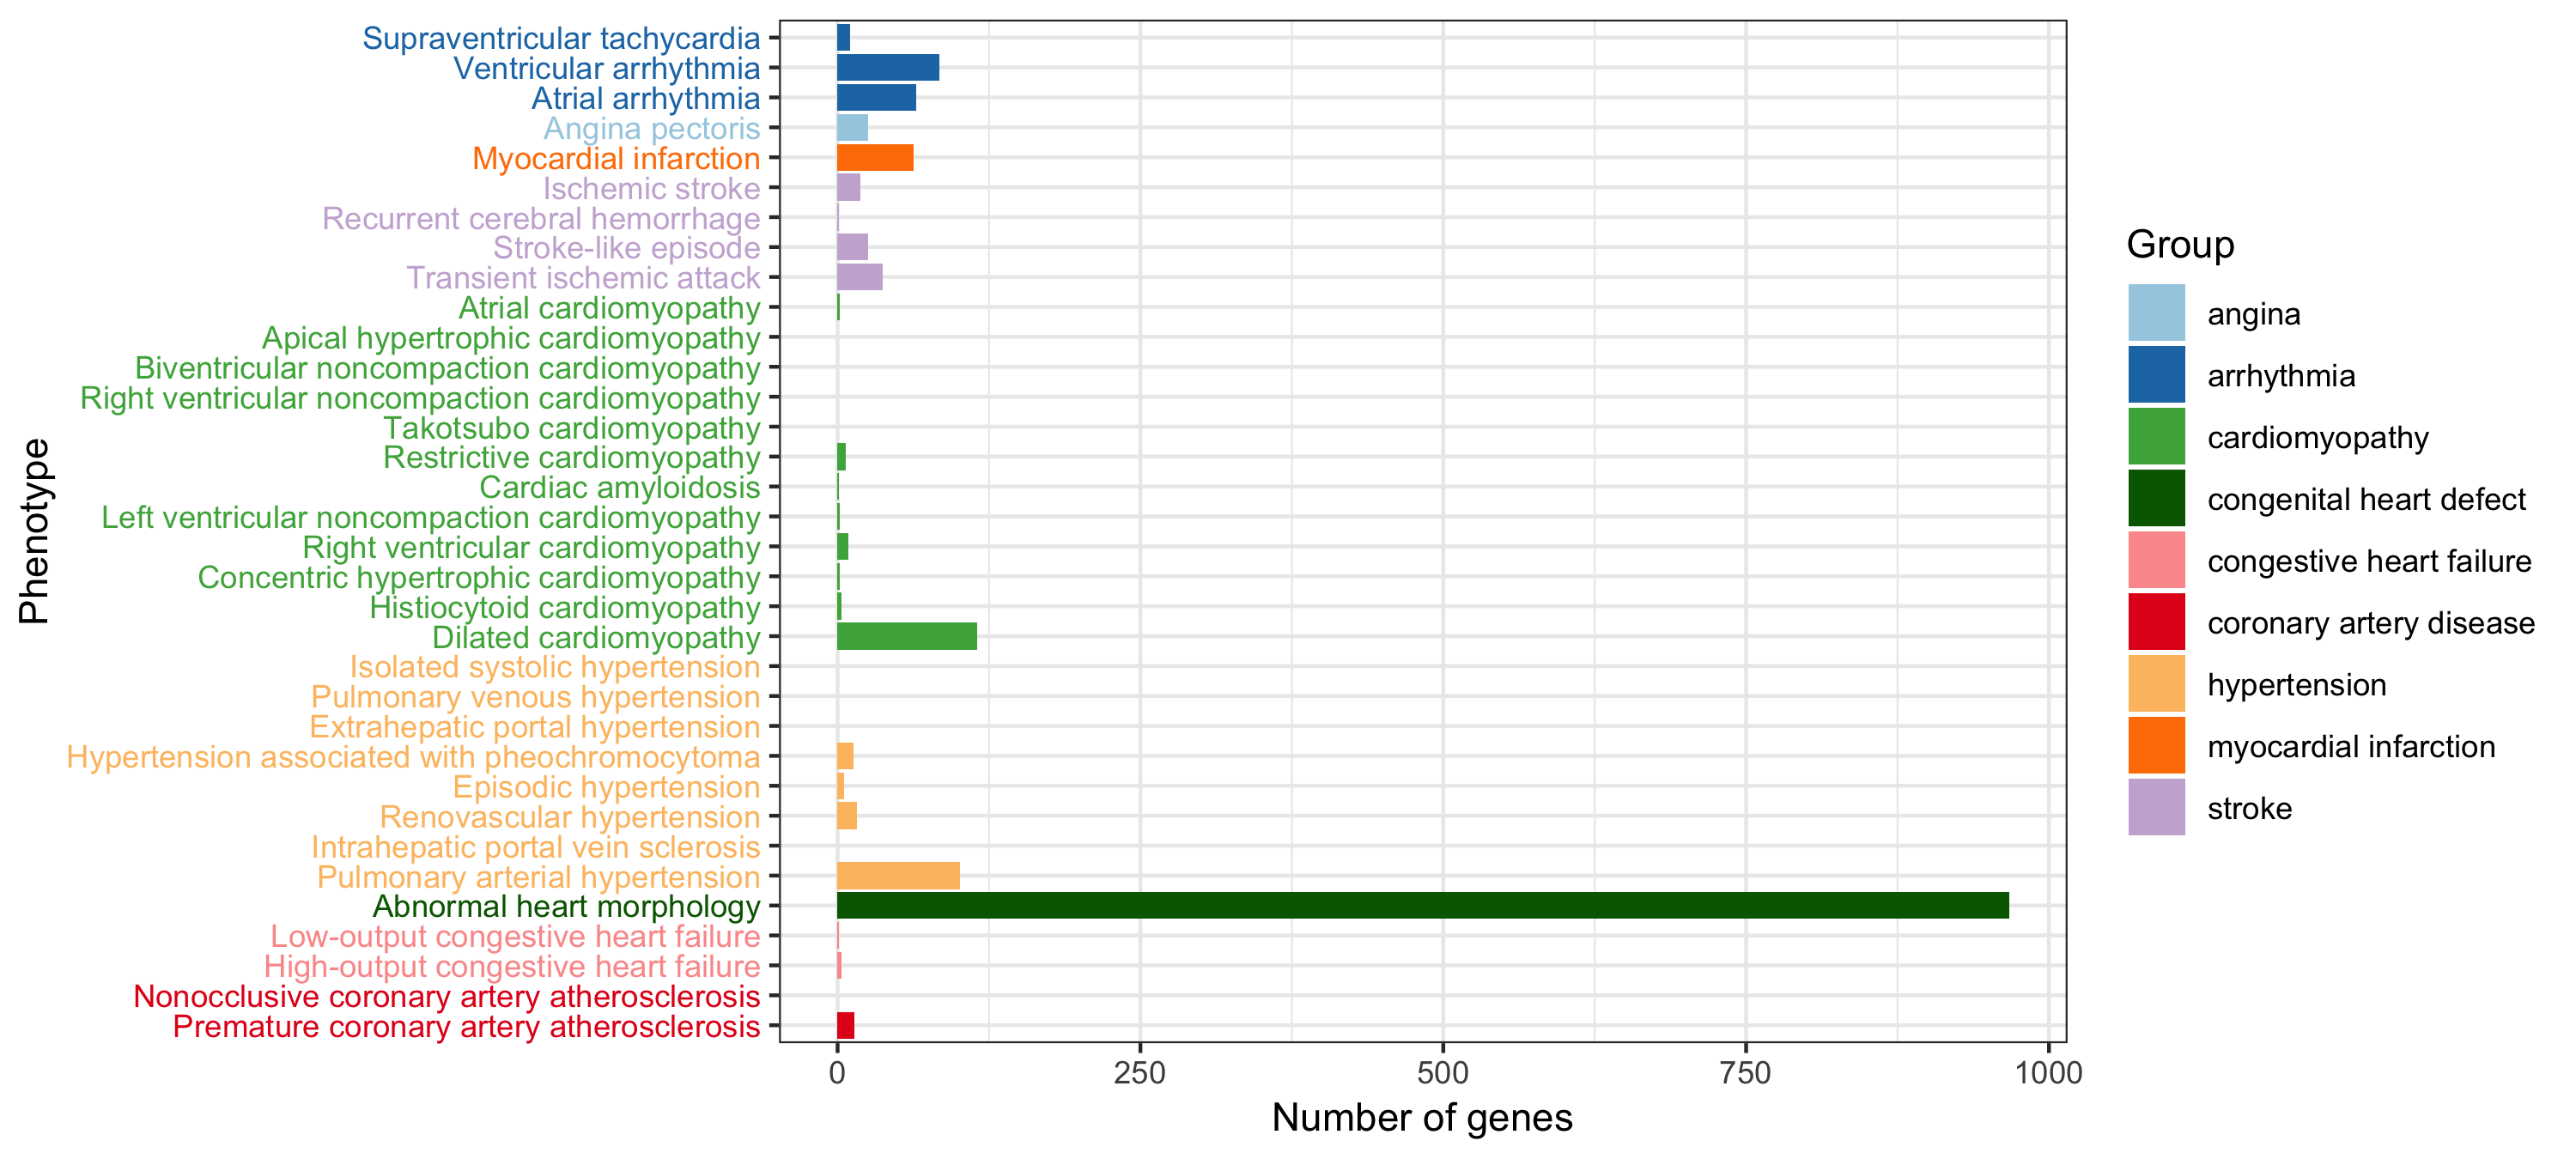
\includegraphics[width=1.\linewidth]{hpo-gene-count}
		\caption{The number of genes associated with \emph{``Abnormality of the cardiovascular system"} (HP:0001626) as reported in the Human Phenotype Ontology \citep{Kohler:2014:Human},
			 with phenotype annotations pooled from OMIM \citep{McKusick:2018:OMIM} , Orphanet \citep{INSERM:1997:Orphanet}  and DECIPHER \citep{Firth:2009:DECIPHER}.}
		\label{fig:hpo_gene_count}	
	\end{figure*}
	
	
	\section*{Complexity of CVDs}  % the problems
	\subsection*{The number of genetic actors}
	
There is a certain genetic component in all major categories of heart disease (Figure \ref{fig:hpo_gene_count}). The increase in genome-wide association studies (GWAS) has led to the associations of more and more variants to human traits and diseases \citep{Visscher:2017:10}, fueling the identification of hundreds of novel drug targets and the development of polygenic risk scores that may help improve our ability to predict a person's pre-disposition to various cardiovascular ailments \citep{Ganna:2013:Multilocus,Goldstein:2014:Simple,Krarup:2015:genetic,Tada:2016:Risk, Abraham:2016:Genomic}, and facilitate early and preventative care \citep{Assimes:2016:Genetic}. Predictably, the number of genetic variants found associated with a disease has also increased and, in most cases, gone beyond a few implicated genes that could be described in a single-page table or diagram.  Dilated cardiomyopathy (DCM), a common cause of heart transplantation \citep{Burke:2016:Clinical}, is a vivid example of how causal variants and their corresponding genes were discovered over the years.  In a recent review \citep{Burke:2016:Clinical}, 16 disease-causing genes were compiled, along with an additional 41 putative genes.  Meanwhile, the NHGRI-EBI GWAS Catalog \citep{MacArthur:2017:new} and annotations on Human Phenotype Ontology \citep{Kohler:2017:Human} suggests a larger number of genes associated with this condition, 69 genes and 115 genes, respectively. Clinical application has been keeping up, with a typical commercial gene panel for DCM genetic testing covering 50 genes on average, and 111 in total \citep{McNally:2017:Dilated}. Although these genes were discovered via different approaches, the catalog of DCM-associated loci kept expanding. Similarly for coronary artery disease, additional loci have been associated with the disease almost every year since 2007, bringing the total number of loci associated with CAD to over 150 \citep{Clarke:2018:GenomeWide}.  Since it is reasonably expected that when more genes are involved in a disease, the individual effect exerted by each gene will be small, these constantly expanding gene panels suggest that the common mutations in a single gene are not likely to capture substantial disease risk for most cases that are polygenic. From a research perspective, these findings imply that the quest of pinpointing causal variants is getting progressively more challenging, because testing the variant-phenotype association on small-effect variations requires a much larger number of samples for sufficient power \citep{Visscher:2017:10}, or critically different methods of statistical testing and inference. Furthermore, as large-scale data becomes more readily available for population-level estimation of many genetic variants with low allele frequencies, the high penetrance of many previously labeled "pathogenic" rare variants (minor allele frequency < 0.1\%) has been questioned \citep{Lek:2016:Analysis}. These observations open up a small window into the complicated and dynamic landscape of human disease genetics.  

Besides the increasing difficulty of discovering these variations, modeling their effects poses another set of challenges. With a potential interaction between every pair of genomic features, be they genes or regulatory sequences, the number of such interactions increases quadratically with the number of actors, leading to the combinatorial explosion of states that a biological system can assume (theoretical calculation: $n$ elements leads to $n(n-1)/2$, i.e. $O(n^2)$ interactions).  The plethora of variants associated with a disease or risk of disease do not promise a quick understanding of pathobiological mechanisms, as the functional consequences of a majority of these variants remain unknown. Among the most understood are PCSK9 \citep{Cohen:2006:Sequence}, ANGPTL4 \citep{Dewey:2016:Inactivating,CARDIoGRAM:2016:Coding}, APOC3 \citep{NHLBI:2014:LossofFunction} on which association tests and sequencing have been combined to ascertain the linkage to coronary artery disease risk, translating to potential vascular protective drugs. The methodology of these studies are still under the influence of mainstream CVD research, i.e. revolving around genotype-phenotype association testing. This top-down approach, i.e. phenotype to gene to variant, has certain limits in its power, requiring more and more samples for less frequent and less penetrant alleles while leaving gaps in mechanistic understanding. Bottom-up approaches in which variations are systematically introduced into a DNA sequence (and their functional consequences are characterized \textit{in vitro}) will complement the current understanding of these diseases. As exemplified in the novel assays enabled by state-of-the-art experimental techniques and computational processing, this approach has demonstrated utility in cancer variant classification \citep{Findlay:2018:Accurate}, foreshadowing similar progress in CVD research.

In addition to the loci that have been directly associated with CVD, a large number of genes or regulatory elements may contribute significantly to CVD risks in an indirect manner, due to highly interconnected biological pathways.  For instance, independent research in aging has unraveled the intertwined relationship between heart disease and longevity pathways \citep{North:2012:Intersection}.  With age being the most important factor in conferring cardiovascular disease risk \citep{Steenman:2017:Cardiac}, it is likely that these longevity genes will be involved in future analyses of CVD genetics. The genetic scope of CVD may be enlarged even further to include most of the genome, under the recently proposed omnigenic model for complex traits, in which most heritability is explained by peripheral genes outside of the core pathways \citep{Boyle:2017:Expanded}. Such expansion calls for a paradigm shift from additive effects of multiple genes to the interactions between them, from the physical genes to the "eigen-genes" that represent biologically functional modules \citep{Weiss:2012:Good}.
	
Such a paradigm shift is, in fact, only part of the potential answer to the long-standing puzzle of missing heritability in cardiovascular disease as well as other complex diseases \citep{Manolio:2009:Finding}. Heritability $H^2$, in the \textit{broad sense}, is the proportion of phenotypic variance that can be explained by genetic factors, while the \textit{narrow sense} heritability $h^2$ is the proportion attributable to additive genetic factors \citep{Manolio:2009:Finding}.
If all the heritability has been accounted for, the squared correlation between the observed and the predicted phenotype should be equal to $H^2$ (or $h^2$). The increasing number of loci associated with complex traits still leave a large gap between predicted and observed phenotypes, prompting different strategies to account for the missing heritability.  One of the more obvious causes of missing heritability relates to the limited ascertainment of the total pool of rare variants in humans. Even among rare causal variants identified to-date, associations with disease has likely been under-appreciated due to insufficient study power to detect modest effects on risk. One addresses this issue by collecting more samples among diverse study populations \citep{Visscher:2017:10, Lek:2016:Analysis} and improving statistical tests \citep{Zuk:2014:Searching,Kaakinen:2017:rarevariant}. Even so, conventional models of phenotype prediction have relied almost exclusively on the additive effects of genetic factors, hence can only explain narrow-sense heritability $h^2$ at best. In addition, alterations outside of DNA sequences have been found to be heritable, suggesting another part of the puzzle relies on epigenetics. Thus, to advance our understanding of complex diseases such as CVD requires moving beyond the exome and genome, as discussed in the next section.
	
	
\subsection*{The diversity of actors}

\subsubsection*{From SNPs to structural variations}

	
	Genome-wide association studies have been predominantly conducted on single-nucleotide polymorphisms (SNPs) thanks to the availability of easy-to-produce SNP microarrays. Such technologies have clearly enriched our knowledge base of the effect of single nucleotide variants, while leaving the effect of structural variations poorly understood. There are now 660 million SNPs documented in the dbSNP database \citep{NCBI:2018:dbSNP}, compared to 4.6 million structural variations in the DGVa (Database of Genomic Variants archive \citep{EMBL-EBI:2018:Database}, which also includes studies annotated by the NCBI-hosted database of structural variants, dbVar \citep{NCBI:2018:dbVar}).  Structural variation (SV) databases such as dbVar and DGVa are in fact storing each study-publication individually instead of cataloging structural variations into data entries. Although the current knowledge base of structural variations is not sufficient to create reference entries of SV, the map of SV from 1000 Genomes Project \citep{Sudmant:2015:integrated} has enabled further studies of the role of SV in cardiac diseases, suggesting the potential impact of SV on the transcriptional regulation of cardiac genes expressed in the heart \citep{Haas:2018:Genomic}. As envisioned, structural variations might be one of the promising areas to look for the missing heritability in CVD \citep{Eichler:2010:Missing}.  To this end, ongoing projects like TOPMed contain a Structural Variant Working Group to call copy-number variants (CNVs) within TOPMed, and they have begun incorporating large-scale multi-ancestry studies spanning diverse types of sequencing data from both European and non-European race/ethnic groups.  
	\begin{figure}[!tpb]
		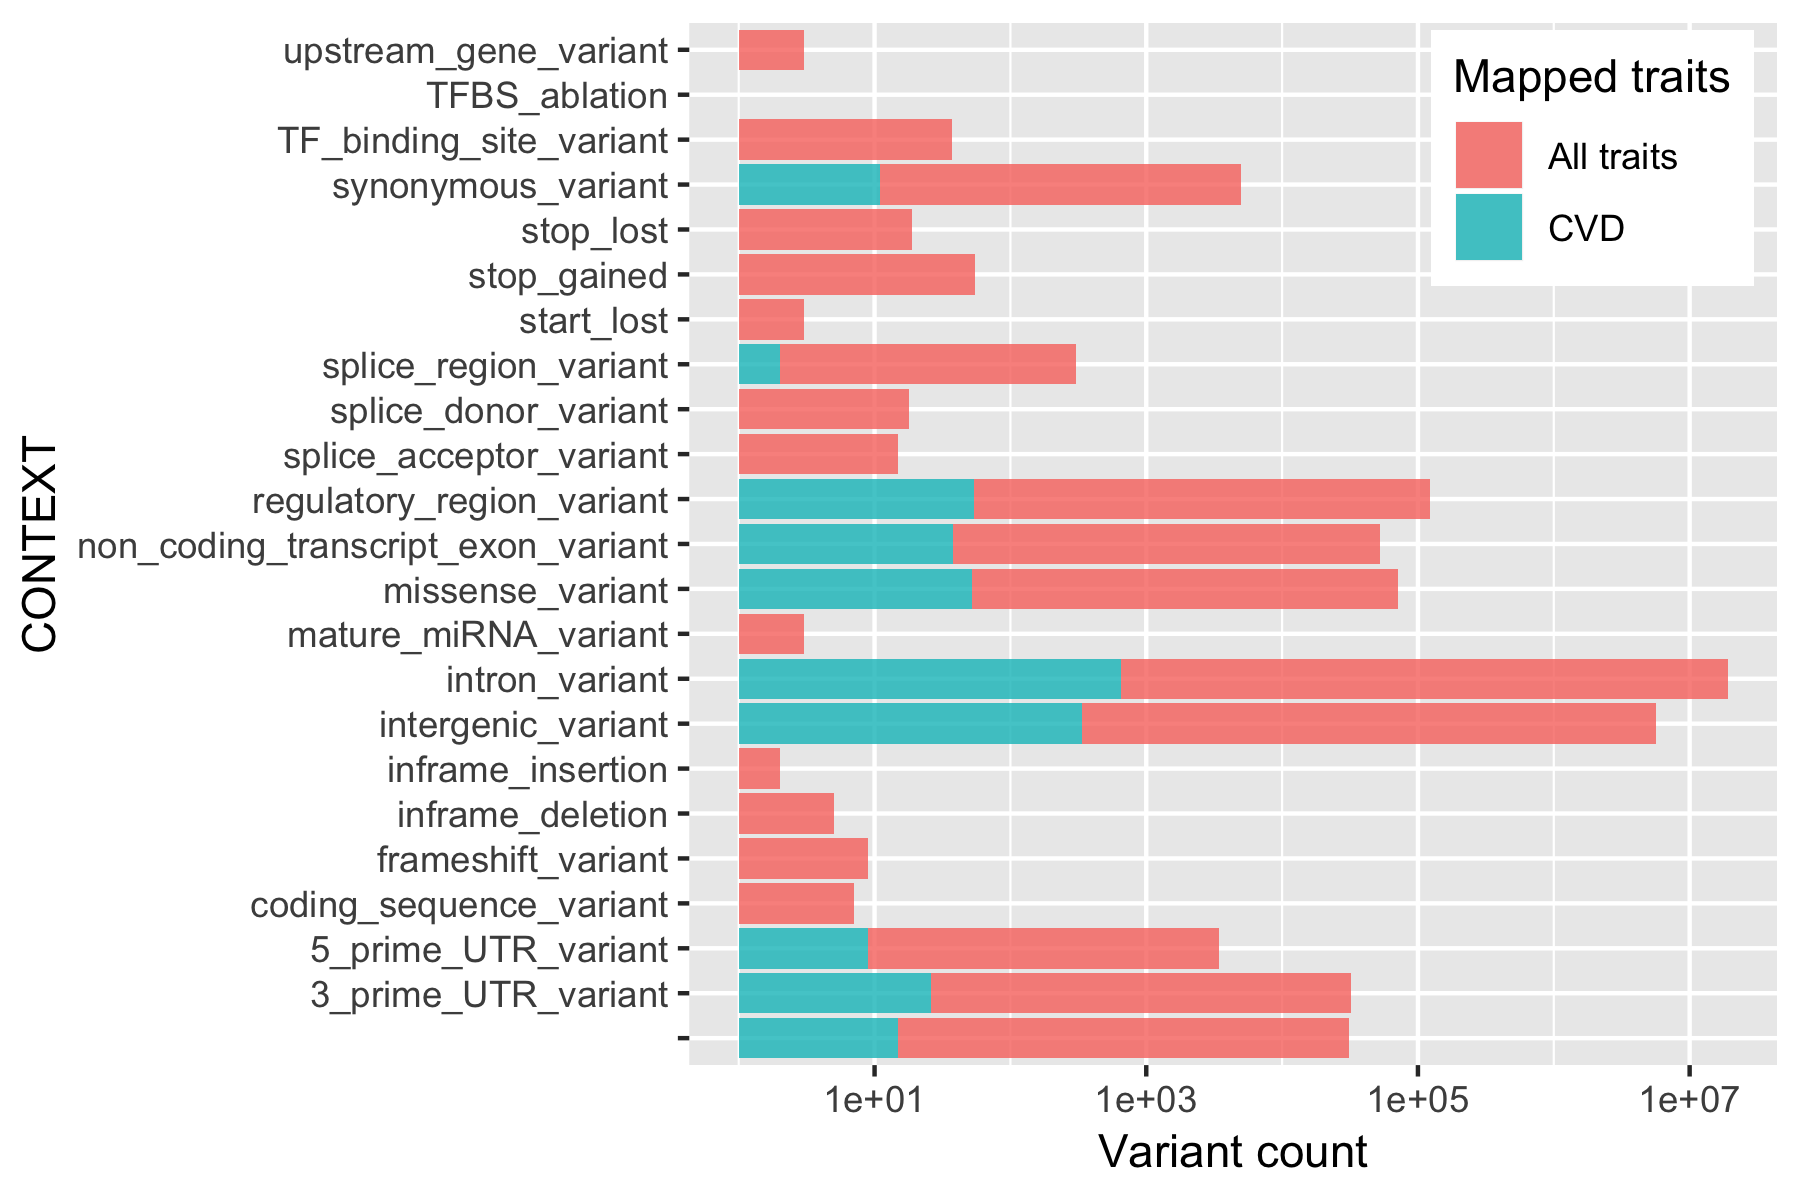
\includegraphics[width=1\linewidth]{variant_contexts}
		\caption{Distribution of SNPs that have been associated with a phenotypic trait in the human genome. The associations are downloaded from NHGRI-EBI GWAS Catalog in which only those with p-value less than $10^{-5}$ were retained.}
		\label{fig:variant_context}
	\end{figure}
	

\subsubsection*{From coding to noncoding regions}	
	As array-based genotyping was gradually replaced by next-generation sequencing, the cost of sequencing an exome, i.e. the protein-coding part of a genome, became much more affordable and enabled the collection of more than 60,000 exomes \citep{Lek:2016:Analysis}. Using this dataset, \cite{Walsh:2017:Reassessment} found that many "pathogenic" genetic variants associated with various cardiomyopathies are equally common in clinical cases as in the control population. Genes that were consistently included on genetic testing panels for DCM such as MYBPC3, MYH6, SCN5A, etc. turned out to be less penetrant than previously thought, in consideration of their frequency in the control population. The rationale for prioritizing the sequencing of exome over that of the entire genome, besides the lower cost, was a regularly cited statement that the exome harbors 85\% of disease-causing variants \citep{Antonarakis:2001:nature} which turned out to be an outdated estimate from 1995. In our own survey of the NHGRI-EBI GWAS Catalog \citep{MacArthur:2017:new}, a large fraction of variants tend to occur in non-protein coding regions such as intronic, intergenic, and splice junctions (Figure \ref{fig:variant_context}). The distribution of CVD-associated variants is similar to that of variants associated with all traits. Previous studies also asserted the prevalence of regulatory regions among variants associated with cardiometabolic risk \citep{Franzen:2016:Cardiometabolic}, as well as many other complex traits \citep{Pickrell:2014:Joint}. As an unprecedented amount of whole-genome sequencing data become available from large-scale genomic projects such as \textit{The 1000 Genomes Project} \citep{1000G:2015:global}, \textit{UK10K} \citep{TheUK10KConsortium:2015:UK10K}, \textit{The 100,000 Genomes Project} \citep{Caulfield:2017:100K}, The \textit{100K Wellness Pioneer Project} in China \citep{Kalia:2017:China}, \textit{All of Us Research Program} \citep{NIH:2018:All}, TOPMed \citep{NHLBI:2014:TransOmics}, and CCDG \citep{NHGRI:2016:CCDG}, we are poised to learn more about this dark matter in the human genome and how it works in complex diseases.

\subsubsection*{Beyond genetics: epigenetics and gene-environment interplay}	
	Cardiovascular risks can be conferred through heritable changes in gene expression without alterations in the underlying DNA sequence.  These epigenetic processes traditionally involve DNA methylation, a wide range of histone modifications including acetylation, methylation, phosphorylation, ubiquitylation, sumoylation and biotinylation, and are now encompassing a loosely-defined group of processes mediated by long noncoding RNAs (lncRNAs). Dysregulation in epigenetic processes has been associated with the pathogenesis of cancer and many other diseases. To date, epigenetic mechanisms have been demonstrated to be involved in a variety of cardiovascular diseases and conditions \citep{Udali:2013:Cardiovascular,AbiKhalil:2014:emerging,Muka:2016:role,Gidlof:2016:Ischemic}.
	For instance, early differential epigenomic analysis, albeit on a limited number of samples, established differentiating features in DNA methylation and histone H3 methylation between control and failing hearts \citep{Movassagh:2011:Distinct}. Following these early findings, epigenome-wide association studies have proposed a number of DNA methylation sites associated with blood lipid \citep{Irvin:2014:Epigenomewide}, body mass index \citep{Dick:2014:DNA, Wahl:2017:Epigenomewide}, heart failure \citep{Meder:2017:EpigenomeWide}, and heart attack history \citep{Rask-Andersen:2016:Epigenomewide}. In addition, alterations in chromatin structure have been shown to induce heart failure \citep{Rosa-Garrido:2017:HighResolution}.  
	
	As more lncRNAs were discovered and characterized, the prevalence of these molecules in cardiovascular biology also emerged.
	At least 22 lncRNAs were reportedly dysregulated in CVDs including coronary artery disease, myocardial infarction, cardiac hypertrophy and atherosclerosis, affecting a wide range of molecular, cellular and physiological processes \citep{Das:2018:Deciphering, Xu:2018:Targeting}. Due to low relative abundance levels and highly tissue-specific expression patterns, lncRNAs remain challenging to study.
	Some of the functions of lncRNA that have been recognized include imprinting, scaffolding, enhancer activity, and molecular sponges. These actions mark the presence of lncRNAs in many cardiovascular processes such as cardiac differentiation, macrophage activation and sarcomere development \citep{Sallam:2018:Long}. With 107,039 lncRNAs detected in the human genome so far (reported by LNCipedia \citep{Volders:2018:LNCipedia}, as of November 2018), more lncRNAs are likely to be implicated in cardiovascular biology, in the future hence promising potential therapeutic targets.


	As epigenetic processes include various molecular and cellular events, the experimental assays for mapping of the epigenome are accordingly diverse. DNA methylation profiling can be done with methylation-sensitive restriction enzymes, bisulfite sequencing, or immunoprecipitation with antibodies against methylated-cytosine \citep{Bibikova:2010:Genomewide}. Histone modifications can be profiled by immunoprecipitation with antibodies specific to the modified histone of interest, essentially requiring a ChIP experiment for each of the histone modifications one wants to interrogate \citep{Kimura:2013:Histone}. Meanwhile, the noncoding RNA transcripts can be profiled with variations of RNA-seq experiments that are optimized for the target fraction of RNA. Such diversity entails significant difficulty in comprehensive profiling of the epigenome in a single experimental assay, stressing the need for re-collection and re-analysis of dispersed datasets for a more complete multi-omics picture. As epigenetic alterations have been found to be responsive to environmental cues throughout life, the epigenome lays an important bridge between the genetic makeup of an organism and its phenotype by helping to explain the gene-environment interplay.
	For example, environmental factors have been known for decades to play critical roles in conferring cardiovascular risk. Framingham-based risk scores \citep{Sheridan:2003:Framinghambased}, which include variables that can be intervened by lifestyle habits (smoking, blood cholesterol, blood pressure, diabetes), have guided clinical practices \citep{British:1998:Joint} and shown to perform well in predicting cardiovascular risk in many populations \citep{Knuiman:1997:Prediction,Eichler:2007:Prediction}. The relative performance of phenotype-based risk scores and the genotype-based counterpart is highly variable depending on specific populations and practices in designing score components. There exist lines of evidence favoring both phenotypic variables \citep{Talmud:2010:Utility} and genotypic ones in predicting disease risk. \citep{DAgostino:2001:Validation,Empana:2003:Are,Eichler:2007:Prediction,Zomer:2014:Cardiovascular}.
	Clearly, there remains a gap in understanding gene-environment interaction that can now be studied at the molecular level, thanks to advances in experimental techniques to measure the exposome, i.e. all environmental exposures throughout life, including an individual's diet, pollutants, and infections \citep{Wild:2005:Complementing}. With recent development of wearable devices to collect real-time data in a non-intrusive manner, it is now possible to monitor the exposome for its dynamic compositions of chemical compounds and micro-organisms \citep{Warth:2017:ExposomeScale, Jiang:2018:Dynamic}. Being amongst complex traits that are heavily influenced by environmental factors, cardiovascular diseases are especially well-positioned to benefit from these advances.
	
	\section*{The challenges of cardioinformatics}
	As illustrated in the previous section, the complexity of cardiovascular diseases calls for pushing research beyond traditional boundaries.
	Such expansion implies the inclusion of various data modalities described above, such as genome sequences, DNA-methylation profiles, RNA expression profiles, protein expression profiles, metabolic profiles, etc. (Figure \ref{fig:trans-omics}) within computational analysis workflows. These modalities represent different classes of biological molecules as well as their interactions (Figure \ref{fig:trans-omics}A). Computational workflows relevant to cardiovascular medicine have been proposed \citep{Ping:2018:Biomedical}, clearly illustrating how CVD research can benefit from existing computing resources, from cloud-computing infrastructures to analytic methods for metadata and search. Likewise, modular data science architectures for supporting cardiovascular investigations have been illustrated \citep{Khomtchouk:2018:HeartBioPortal,Scruggs:2015:harnessing}.  Due to the sheer amount of data obtained from CVD research, ranging from medical records to medical images and high-throughput omics profiles, challenges related to data management and analysis that are generic to many fields become even more pressing for cardioinformatics. While benefiting from two decades of research in bioinformatics, there remain significant challenges that can be addressed to accelerate CVD research. From our own perspective, we suggest three particularly pertinent areas to prioritize cardioinformatics research: data sharing/security, multi-omics analysis, and augmented intelligence.
	
	
	\subsection*{To share or not to share}
	Data sharing is believed to help scientific advances, thus benefiting everyone \citep{GA4GH:2014:Framework}. The sharing of personal health and medical data, however, comes with the risk of compromising a person's privacy and subjecting them to discrimination \citep{P3gConsortium:2009:Public,GA4GH:2014:Framework,Shringarpure:2015:Privacy}.  The current data governance practices employ several administrative measures in the hope of minimizing the risk of exposing the data to adversity, or bad intentions. Taking the process of dbGaP data requests as an example: to access 658,305 records of genotype-phenotype data (Table \ref{tab:dbgapSubject}) potentially relevant to future biomedical studies, a researcher first needs to browse these datasets, determine whether each dataset is consented for its purpose, obtain IRB approval if necessary, then file a request, prepare the facility, implement the security measures, and transfer the data upon approval. Although the data users are advised, for example, to "avoid placing data on mobile devices" and "destroy [the data] if they are no longer used or needed", the only guarantee to such compliance is the vigilant mindset of every researcher involved in the data behind the project(s).  In addition, datasets are associated with different types of consents, dictating what purposes are permitted (e.g., general research, disease-specific research, or biomedical research). Therefore, data users are responsible for obtaining the IRB approval compatible with these consents. These regulatory requirements have heightened the barrier to data access without robust mechanisms to enforce data protection nor to revoke the access when necessary.  To add to these challenges, before filing a request, one needs to dive into the metadata of individual studies and decide which datasets are useful for the target research. Important information about a dataset such as the list of phenotypic variables are often vastly different from study to study and cannot be filtered against. In addition to those parameters of a study design, researchers need to be aware of the various types of consent forms applied to different datasets, many times within a single study. This procedure to obtain data access is currently applied for all controlled-access data in dbGaP, adding a significant administrative burden to biomedical researchers.

	As a pioneering effort towards more accessible biomedical data, the AHA's Precision Medicine Platform \citep{Kass-Hout:2018:American} has greatly simplified this process by streamlining the search, request and transfer of data. Datasets deposited on this platform were harmonized such that users can query for data across multiple studies by some common parameters, selectively request access to the relevant data, and perform analyses on the cloud-based workspace. The platform has lifted significant burden off of data users by having them file one request for multiple datasets, and the data owners, being aware and responsible for complying with the consents on their data, will decide whether access can be granted or not. The cloud-based workspace also allows data to be transferred and analyzed in a controlled environment that can be ensured to comply with regulatory standards. The risk of intellectual property being compromised remains, for the data, once transferred, cannot be withdrawn nor prevented from being copied. As recognized by the authors, the platform is "only as good as the researchers make it" \citep{Kass-Hout:2018:American}.
	More secure modes of data sharing have been explored, forming a spectrum of varying balance between analytic power and data protection. ViPAR \citep{Carter:2016:ViPAR} supports on-memory analysis of pooled data that is transferred to a central system, avoiding the permanent storage of sensitive data outside of the original sites.  In all of the platforms above, a strong system for registering users as well as applying sanction measures are critical to enforce data usage agreements and deter malicious intent. Nevertheless, there still remains significant risk associated with data transfer and data protection at the user end.
	A couple of solutions have been proposed to further reduce the risks and responsibilities associated with direct access to sensitive data. For example, PRINCESS \citep{Chen:2017:PRINCESS} is designed to perform statistical tests within an enclave hosted on a trusted server, in a stream of small data segments (8000 SNPs at a time). On the other end of the spectrum, DataSHIELD \citep{Gaye:2014:DataSHIELD, Wilson:2017:DataSHIELD} and COINSTAC \citep{Plis:2016:COINSTAC} aim to allow data to be analyzed without moving out of the owners' facility. Current implementations have shown that a variety of analytic tasks such as summary statistics, histogram, generalized linear model (DataSHIELD), and gradient descent (COINSTAC) can be performed in a distributed manner to achieve equally accurate results compared to the physically pooled counterpart and, more importantly, without disclosure of sensitive or personally identifiable information.
	
    Besides controlled-access data, a large amount of publicly available human data such as RNA-seq, ChIP-seq, Hi-C, etc. results are freely accessible with no restriction. Without genomic sequences, genotype or phenotype data, the processed output of these assays are deemed anonymous and void of sensitive information. However, recent studies have shown that information leakage is still possible, subjecting individuals to linking attacks that may reveal their identity \citep{Harmanci:2016:Quantification, Harmanci:2018:Analysis}.  With millions of human genomes and thousands of other omics profiles on the not-so-distant horizon, a large fraction of which comes from CVD research programs (Figure \ref{fig:trans-omics}), it is critical that cardioinformatics researchers pioneer the applications of these security measures, to ensure scientific advances do not compromise human rights to privacy and non-discrimination.
	
	\subsection*{Multi-omics data ocean}
    The explosion of biological data is manifested in the growth of databases, consortium efforts, repositories, as well as the amount of raw and summary-level data hosted in these warehouses. High-throughput technologies are now available for characterizing and quantifying all major classes of biological molecules including DNA, RNA and protein (Figure \ref{fig:trans-omics}A), leading to the creation of centralized repositories such as the Gene Expression Omnibus (GEO) \citep{Barrett:2013:NCBI} for gene expression data, dbGaP \citep{Tryka:2014:dbGaP} for genotypes and phenotypes, ProteomeXchange \citep{Vizcaino:2014:ProteomeXchange,Deutsch:2017:ProteomeXchange} for proteomics, MetabolomeXchange for metabolomics, among others.  GEO, one of the most popular repositories for functional genomics data, has accumulated more than 100,000 datasets \citep{Zhu:2008:GEOmetadb}. Among these, CVD publications have contributed more than 2000 microarray-based experiments, and about 900 high-throughput sequencing experiments for various purposes (Figure \ref{fig:geo-assay}). The amount of data potentially re-usable for CVD research may be even larger, when taking into account studies that did not focus on cardiovascular disease but generated a decent number of assays on relevant biospecimens (e.g., heart, blood or blood vessels) such as ENCODE \citep{ENCODE:2012:integrated} and the Roadmap Epigenomics initiatives \citep{Roadmap:2015:Integrative}.
	Likewise in dbGaP, where human genotype-phenotype data are deposited, CVD-related research has contributed data on 658,305 subjects, only 16,786 (2.5\%) of whom had consented for the data to be employed for general research, leaving a large amount of data locked in field-specific or disease-specific studies (Table \ref{tab:dbgapSubject}) (see Supplementary information for a comprehensive list of CVD studies deposited in dbGaP). Future studies seeking to take advantage of these data are subjected to a significant administrative barrier to explore, access and make use of the data, as described in the previous section.
	In addition to the central repositories for established and popular experimental methods, smaller databases with narrower focus are also budding. For instance, chromatin structure data from 3C, 4C, 5C and Hi-C experiments have been collected in dedicated databases such as 3CDB \citep{Yun:2016:3CDB} and 4DGenome \citep{Teng:2015:4DGenome}. Also, noncoding RNAs are being added into databases such as lncRNAdb \citep{Quek:2015:lncRNAdb}, NONCODE \citep{Fang:2018:NONCODEV5}, and LNCipedia \citep{Volders:2018:LNCipedia}.
	
	
			\begin{table}[]
	\processtable{The subject count aggregated from studies deposited in dbGaP, consented for General Research Use (GRU)
		\label{tab:dbgapSubject}}
{\begin{tabular}{l l l}
			\toprule
			& \textbf{CVD} &  \textbf{All}                         \\ \midrule
			16s rRNA (NGS)                 &     0 &      92 \\
			CNV Genotypes                  &     0 &   48972 \\
			Chromatin (NGS)                &     0 &     139 \\
			Genomic Sequence Amplicon (NGS)&     0 &       8 \\
			Methylation (CpG)              &     0 &     657 \\
			Methylome sequencing           &     0 &     152 \\
			QTL Results                    &     0 &     281 \\
			RNA Seq (NGS)                  &   333 &    1498 \\
			SNP Genotypes (Array)          &  6658 &  113597 \\
			SNP Genotypes (NGS)            &  4277 &   11786 \\
			SNP Genotypes (PCR)            &     0 &      10 \\
			SNP Genotypes (imputed)        &     0 &   29693 \\
			SNP/CNV Genotypes (NGS)        &     0 &     936 \\
			SNP/CNV Genotypes (imputed)    &     0 &    9291 \\
			SNV (.MAF)                     &     0 &       2 \\
			SNV Aggregate (.MAF)           &     0 &     570 \\
			Targeted Genome (NGS)          &     0 &    9918 \\
			Whole Exome (NGS)              &  5518 &   12771 \\
			Whole Genome (NGS)             &     0 &    1245 \\
			mRNA Expression (Array)        &     0 &     798 \\
			miRNA (NGS)                        & 0 &   228 \\ \hline
			Total subject count in data consented for GRU & 16786 & 242644 \\ \hline
			All consent groups & 658305 & Unknown \\	
		\end{tabular}}{NGS: Next-generation sequencing\\ QTL: Quantitative Trait Loci}
	\end{table}
	
	Such abundance and diversity of data promises valuable insights once the data is aggregated across studies within a given omics domain (e.g., RNA-seq), or across multiple omics domains (e.g., RNA-seq, ChIP-seq, ATAC-seq, etc.). Efforts to aggregate genomic data (both individual and summary-level statistics) have resulted in valuable collections such as The Cancer Genome Atlas \citep{TCGA:2013:Cancer} for genomics and functional genomics data in cancer, or ExAC and gnomAD for exome and genome sequencing data \citep{Lek:2016:Analysis}. For instance, aggregated exomes/genomes such as ExAC/gnomAD have been a valuable resource for estimating the allele frequencies of the general population as well as within various race/ethnic groups. With the upcoming wave of trans-omics data spanning diverse populations and sequencing types (Figure \ref{fig:trans-omics}B), data harmonization will become a more pressing problem for cardioinformatics. Some early solutions have started to be proposed, e.g., Biochat for GEO metadata \citep{Khomtchouk:2018:Biochat} or OmicsDI for diverse datasets spanning genomics, transcriptomics, proteomics and metabolomics \citep{Perez-Riverol:2017:Discovering}.
	
	\begin{figure*}[!tpb]
		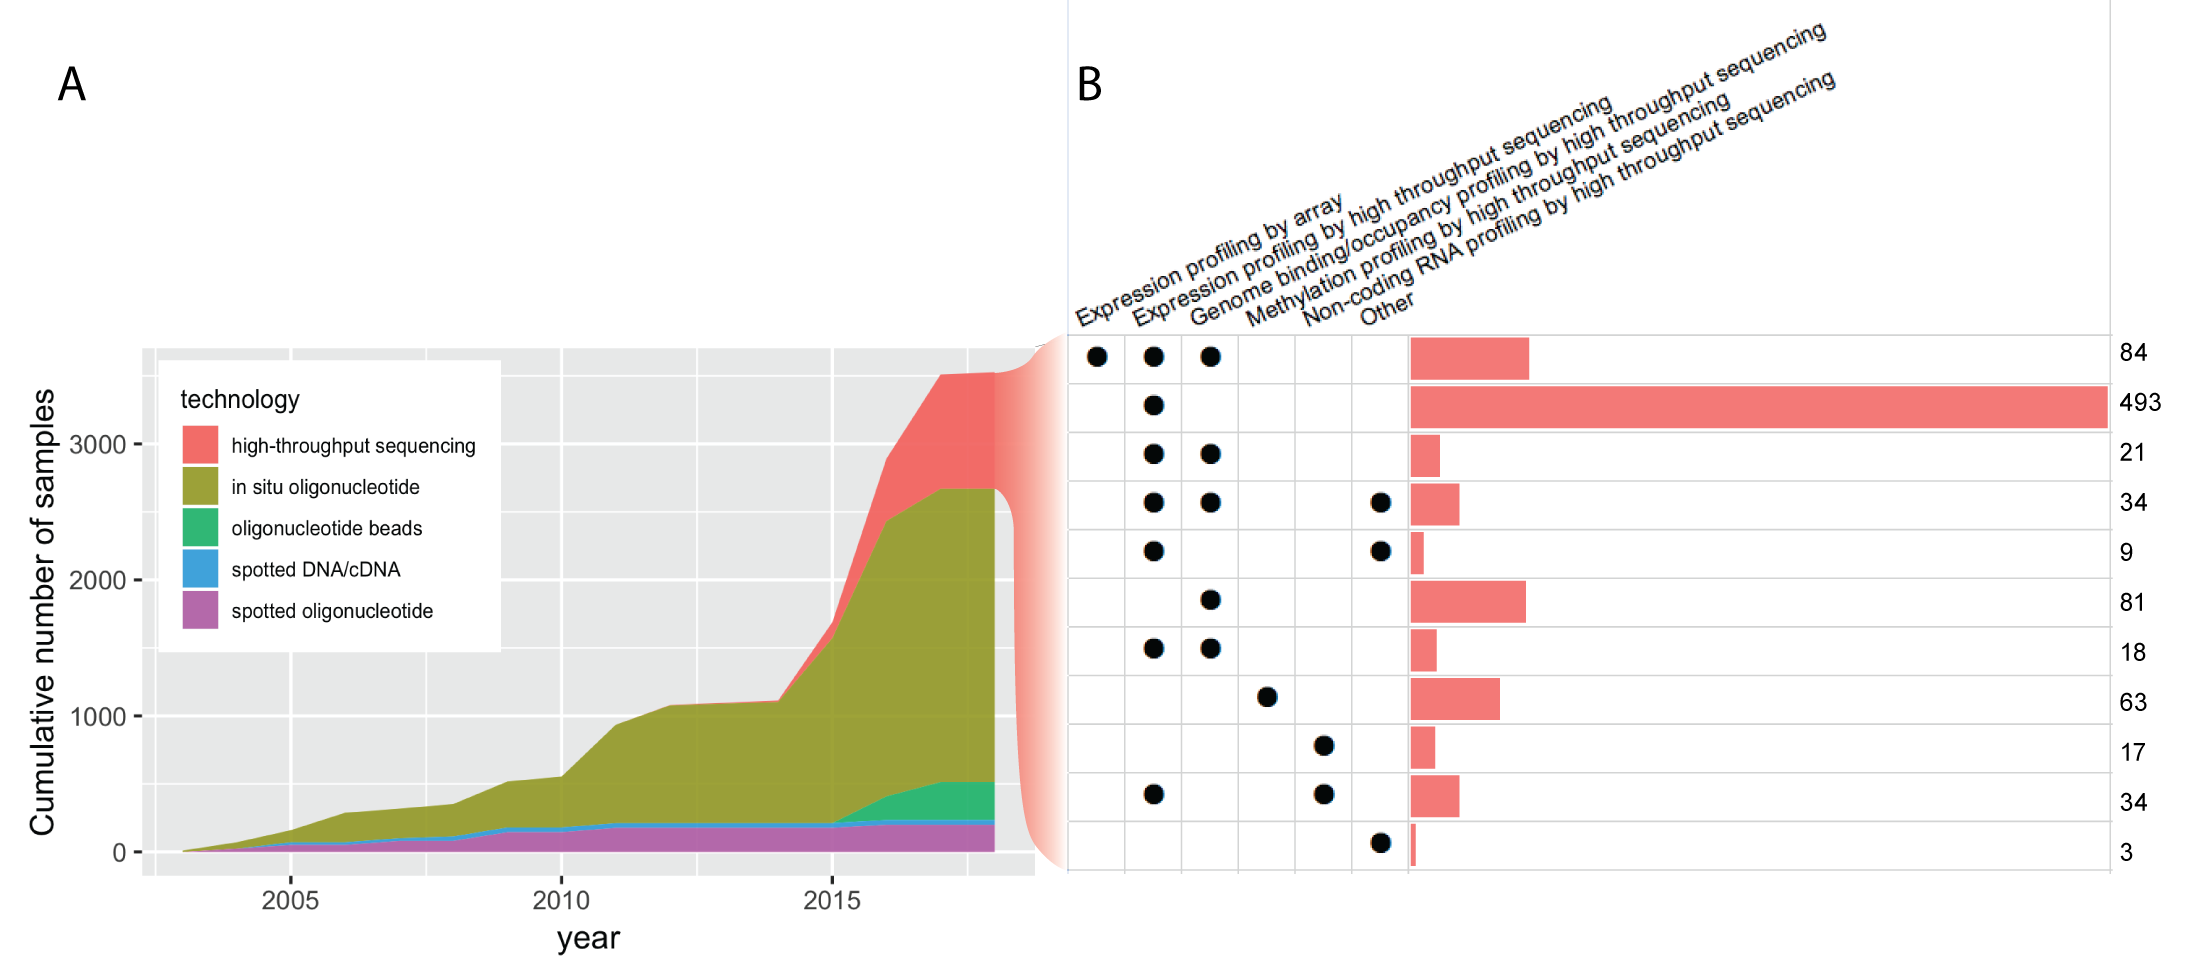
\includegraphics[width=1\linewidth]{assay-count-cardio}
		\caption{(\textbf{A}) The cumulative number of molecular assays (i.e. unique combinations of biosample, study and platform) deposited in GEO by cardiovascular research. (\textbf{B}) Breakdown of high-throughput sequencing assays by the type of study. Expression profiling by high-throughput sequencing, i.e. mRNA-seq assays, are often coupled with another profiling technique, for example, to provide functional read-out of transcription factor binding profiled by ChIP-seq. \label{fig:geo-assay}\\ Note that to avoid excessive over-counting of irrelevant samples such as those from plants or unrelated model organisms, we only counted samples deposited with a PubMed ID pointing to a cardiovascular study. Surveys were done on the GEOmetadb database \citep{Zhu:2008:GEOmetadb} updated on 2018/11/17.}
	\end{figure*} 
	
	While the issues above are generic for all types of research aiming to re-use public data, we believe CVD research benefits even more by expanding beyond traditional methods. Most use of high-throughput data in CVD research has been largely limited to the very first layer of omics data (Figure \ref{fig:trans-omics}A), i.e. genome/exome. Whole-exome and whole-genome sequencing data have been slowly incorporated into conventional GWAS, bringing more ascertainment to earlier findings \citep{Cohen:2006:Sequence,Dewey:2016:Inactivating,CARDIoGRAM:2016:Coding,NHLBI:2014:LossofFunction}. When deeper phenotype data such as blood lipid tests and diagnosis (ICD) codes became available, phenome-wide association studies (PheWAS) emerged \citep{Denny:2013:Systematic}, triggering a new line of biomedical research that coupled electronic health records (EHRs) with omics data, enabling powerful analyses, as discussed by  \cite{Denaxas:2015:Big, Wu:2017:Omic} and exemplified by \cite{Dewey:2016:Distribution,Li:2018:Decoding}. 


    	\begin{figure*}[!tpb]
	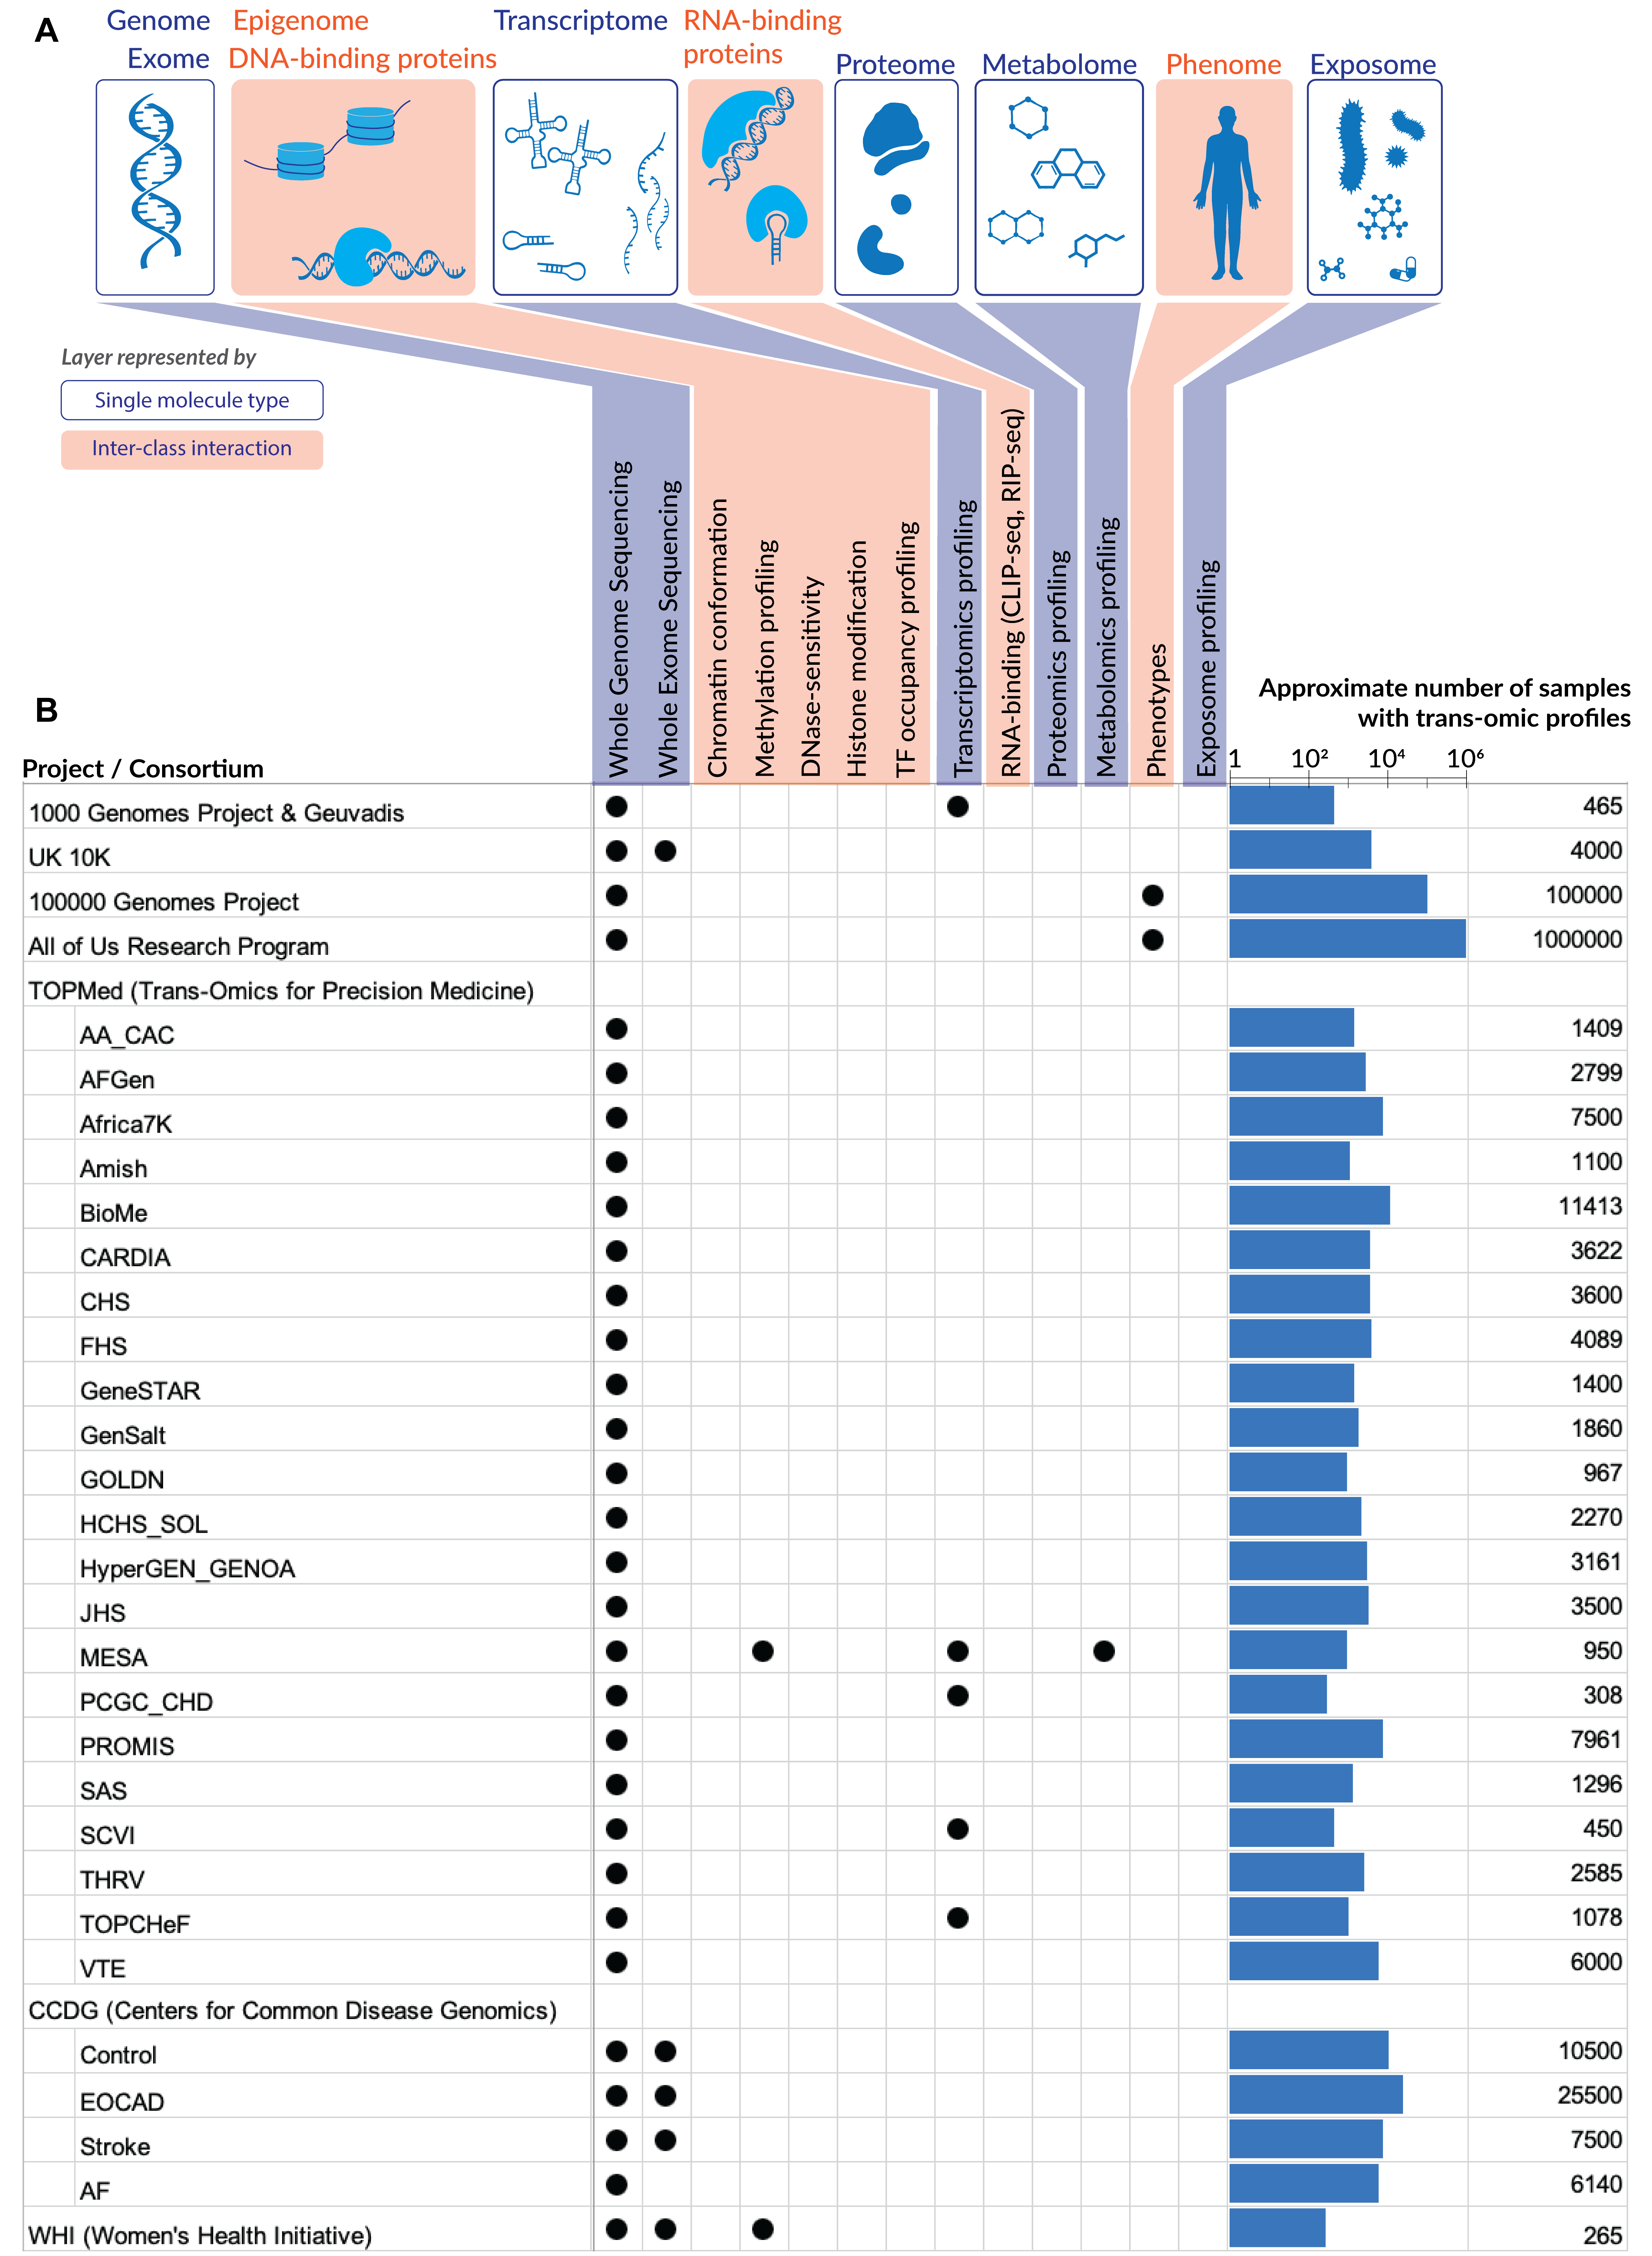
\includegraphics[width=0.9\linewidth]{trans-omics-data-sets.png}
		\caption{ (\textbf{A}) The multiple layers of omics data that are now accessible to researchers. Genome/exome, transcriptome, proteome, metabolome, as well as the microbiome and chemical compounds in the exposome can be profiled by assays on a single class of molecules (DNA, RNA, proteins or small molecules), while the other layers depend on the ability to capture DNA-protein or RNA-protein interactions. The phenome is less well-defined as phenotypic measures vary greatly from physical measurements to lab tests, from descriptive to quantitative traits. Sources of comprehensive phenotypic data comparable to the other omics can be obtained, for example, from electronic health records.
		Beyond the genome, omics datasets become highly complicated, due to the variation across tissues and cell types.
		(\textbf{B}) Large omics datasets that are (or will be) available for CVD research. For each dataset, the number of samples being assayed across multiple omics are indicated on the right. This number is often smaller than the total number of samples/participants in a given project, because not every sample is run on multiple assays.}
		\label{fig:trans-omics}
	\end{figure*} 
	
	
	Besides existing data, new recent research programs have started to put more focus on high-throughput assays that result in a comprehensive cross-section of biological molecules (DNA, RNA and protein) and their interactions. For instance, the Multi-Ethnic Study of Atherosclerosis (MESA) medical research study \citep{Bild:2002:MultiEthnic} within TOPMed includes WGS, RNA-seq, metabolomics, proteomics, and methylomics data across a variety of multi-ethnic communities (white, Hispanic, African-American, and Asian).  Specifically, MESA investigates the characteristics of subclinical cardiovascular disease (disease detected non-invasively before it has produced clinical signs and symptoms) and the risk factors that predict progression to clinically overt cardiovascular disease or progression of the subclinical disease.  Likewise, TOPMed is generating a second modest size multi-omic resource involving RNA-seq, metabolomics, and methylomics in a subset of participants of the Women's Health Initiative (WHI) study \citep{NHLBI:1991:Women} who have undergone whole genome sequencing already.  
	 Figure \ref{fig:trans-omics} highlights the large datasets that are (or will be) available for cardiovascular research. It is clear that assays for DNA sequences, including whole-genome sequencing and whole-exome sequencing, are still dominant among these studies. However, a modest number of multi-omics experiments are planned to be assayed for transcriptome, methylome, and metabolome, as in the MESA and WHI studies. The availability of these datasets, especially at the individual-level, is critical to correlate the variations across multiple omics and bridge the gap from genotype to phenotype.  In general, the analysis of these trans-omics datasets is a fascinating problem -- although the computational approaches envisioned from the early days of gene expression profiling, i.e. differential gene expression analysis, co-expression analysis and gene clustering with subsequent identification of enriched biological pathways \citep{Claverie:1999:Computational} can still bring fruitful analysis \citep{Santolini:2018:personalized}, cardioinformatics is clearly steering towards the integration of multiple omics layers (Figure \ref{fig:trans-omics}). Nevertheless, the potential of data integration had been recognized as early as a decade ago (\cite{Hawkins:2010:Nextgeneration}), leading to the development of many data integration strategies \citep{Ritchie:2015:Methods}. Successful data integration, for example of gene expression and summary-level associations of SNPs and phenotypes from GWAS studies, has emerged only recently in CVD research \citep{Gusev:2016:Integrative}. Such approaches, usually referred to as transcriptome-wide association studies (TWAS), are now adopted more widely \citep{Klarin:2018:Genetics}.  Historically, although the first draft of the human genome project had brought a lot of hope and excitement about potential advancements in the diagnosis and treatment of cardiac diseases -- such as the ability to identify disease genes within the associated loci, to improve risk estimation based on more precise genotypes, or to personalize the prediction of drug effects on a patient \citep{Komajda:2001:heart} -- it seems that a collection of the first "drafts" of the whole "multi-ome" will ultimately be required for gaining a deeper understanding of the phenotypic manifestations of CVD across different race/ethnic groups.  A recent cardiac hypertrophy study in mice \citep{Lau:2018:integrated} highlighted the utility of conducting multi-omics investigations for discovering additional disease gene candidates not apparent from studying each omics data type separately in the context of CVD pathogenesis.  All in all, the ability to combine data from every omics layer depicted in Figure \ref{fig:trans-omics}, either at the summary-level or the individual-level, opens up ample opportunities for cardioinformatics to expand and augment the understanding of cardiovascular disease etiology.
	
	
	\subsection*{Augmented intelligence to advance cardiology}
	As alluded to in the Introduction, AI and machine learning will play an increasingly important role in cardioinformatics research.  Recent trends in this direction include studies for cardiac arrhythmia detection \citep{Hannun:2019:Cardiologist}, heart failure prediction and classification \citep{Awan:2018:Machine,Choi:2017:Using,Shah:2015:phenomapping}, cardiovascular risk stratification \citep{Singh:2011:Acomparison}, among various other active CVD research areas \citep{Johnson:2018:Artificial,Alaref:2018:Clinical,Krittanawong:2017:Artificial} that utilize ML techniques ranging from deep learning \citep{Hannun:2019:Cardiologist,Bizopoulos:2018:Deep,Madani:2018:Deep,Lee:2018:Deep,Kwon:2018:Algorithm,Choi:2017:Using}, class imbalance learning \citep{Liu:2014:Risk,Rahman2013AddressingTC}, active learning \citep{NIPS2010_4091}, probabilistic graphical models \citep{Orphanou:2016:DBN,Gong:2015:Inferring}, etc.  But in an era of big data and an accelerated adoption of machine learning methodologies, the role of human experts may turn out to be even more indispensable. Among tasks that still require considerable human judgment include understanding and processing of free text data as well as recognizing visual patterns, especially corner/edge cases (e.g., in CVD medical imaging \citep{Slomka:2017:Cardiac,Fonseca:2011:Cardiac}) that may be missed by algorithms trained on conventional datasets.  As with other areas, cardiovascular research requires expert level domain knowledge to make the best use of machine learning applications, for instance in properly labeling CVD data or harmonizing it across epidemiological cohorts.  Without a doubt, domain expertise in cardiology is by no means a tractable problem at scale, exemplified by the insurmountable pile of cardiovascular publications accumulating over the years (Figure \ref{fig:figure1}B) and the intrinsic difficulty in keeping up with this momentum.  With active research in text-mining and natural language processing (NLP), the goal is to liberate human researchers from the time-consuming tasks associated with reading new CVD literature and making sense of free texts in metadata and publications at scale, including tables, figures, and charts.  Recently, a novel text-mining NLP-based approach was used to analyze over 1 million literature abstracts to uncover novel extracellular matrix functions, pathways, and molecular relationships implicated across six cardiovascular diseases \citep{Liem:2018:phrase}.  Since different subdomains in biomedical literature vary along many linguistic dimensions, making text mining systems that perform well on one subdomain not guaranteed to perform well on another \citep{Lippincott:2011:Exploring, Kilicoglu:2018:Biomedical, Khomtchouk:2018:Biochat}, we believe that development of cardioNLP algorithms and dedicated large-scale comprehensively labeled CVD training datasets will be essential for progress in tasks such as harmonized patient-data meta analyses in cardiovascular precision medicine.  
	
	Recognition of visual patterns, on the other hand, remains a powerful human faculty that needs to be fully exploited rather than entirely replaced with automation.  With the rise of various visualization techniques across diverse biological data types \citep{Pavlopoulos:2015:Visualizing,ODonoghue:2018:Visualization}, it will be an exciting challenge for cardioinformatics researchers to leverage them for an integrative representation of heterogeneous data layers towards extracting deeper CVD insights. In addition, the visualization of many experimental assays and biological processes remains a significant challenge, e.g. visualizing alternative splicing events \citep{Katz:2015:Quantitative,Strobelt:2016:Vials}, fast implementations for biological heatmaps \citep{Khomtchouk:2017:shinyheatmap} or interactive matrices for chromatin conformation data from Hi-C experiments \citep{Kerpedjiev:2018:HiGlass,Lekschas:2018:HiPiler}. Moving into the clinical setting, gearing up towards large-scale precision medicine will entail the requirement of providing more comprehensive and integrated data, in a more comprehensible manner to assist clinicians.  To this end, visualization technology and software design will be critical in improving CVD biomedical software, e.g., for designing robust clinical decision support systems or validating prediction models for critical care outcomes.  For instance, by integrating multiple measures of clinical trajectories together with NLP of clinical free text notes from electronic health record data, more accurate prediction of critical care outcomes were observed among patients in intensive care units across three major hospital systems \citep{Marafino:2018:Validation}.  Such studies suggest that automated algorithms, particularly those using unstructured data from notes and other sources, can augment clinical research and quality improvement initiatives.
	
	
	\section*{Closing remarks}
	As we further our quest to understand the genetics and molecular biology of heart disease, many complex clinical indications have become too complicated for traditional approaches. Reflecting on the current body of knowledge, we recognize that many aspects of this complexity can be addressed with more (and improved) computational methods, as has been the case for bioinformatics in cancer genomics research.  But bioinformatics is more than just a powerful toolkit of techniques for conducting high-end cardiovascular disease studies, as many important perspectives have arisen from the application, development, and expansion of advanced computational methodologies in this area.  In this review, we discussed some of the important work evolving at the multidisciplinary interface of bioinformatics and cardiology, and advocate for shining a brighter spotlight on cardioinformatics as an emerging field, in its own right.  We suggest some future insights based on our understanding of historical perspectives and ongoing work in current CVD research, and welcome feedback and ideas from the broader scientific community.

	\enlargethispage{12pt}
	
	
	
	
	\section*{Acknowledgements}
	
	BBK acknowledges and thanks the American Heart Association (AHA) for financial support through the AHA Postdoctoral Fellowship program.
	\vspace*{-12pt}
	
	\section*{Funding}
	
	This work has been supported by the American Heart Association (AHA) Postdoctoral Fellowship grant \#18POST34030375 (Khomtchouk) and partially by the National Science Foundation [CAREER grant 1350344 to M.M.]. The U.S. Government is authorized to reproduce and distribute reprints for Governmental purposes notwithstanding any copyright notation thereon.\vspace*{-12pt}
	
	\section*{Competing interests}
	
	BBK is a co-founder of Quiltomics, and Research Associate at the VA Palo Alto Health Care System (Million Veterans Program).  OG is a co-founder of EpiCypher, Inc. and Athelas Therapeutics, Inc.  The other authors report no conflicts.\vspace*{-12pt} 
	
	\bibliographystyle{natbib}
	%\bibliographystyle{achemnat}
	%\bibliographystyle{plainnat}
	%\bibliographystyle{abbrv}
	%
	%\bibliographystyle{plain}
	%
	\bibliography{cardio}
	
	
	
\end{document}